\documentclass[conference]{IEEEtran}

\usepackage{cite}
\usepackage{amsmath,amssymb,amsfonts}
\usepackage{graphicx}
\usepackage{hyperref}

\title{Unsupervised Detection of Attack Surface Drift\\
\large CS 4412 Project Proposal}

\author{
\IEEEauthorblockN{Alec Sundby, Tiffany Strickland, Elvin P}
\IEEEauthorblockA{
CS4412 ASM Data Mining\\
Kennesaw State University\\
asundby@student.kennesaw.edu
}
}

\begin{document}

\maketitle

This proposal outlines our project to apply unsupervised data mining to the field of Attack Surface Management (ASM). We are using the LANL Cyber Security dataset to find patterns of software drift and Shadow IT that standard security tools often miss. We are going to use PCA for dimensionality reduction, DBSCAN for clustering, and Isolation Forests to find statistical outliers in network telemetry. These three tactics work together as a pipeline. PCA acts as the first layer to compress the high-dimensional logs, which makes it feasible for DBSCAN to identify behavioral clusters. The Isolation Forest then processes the data to rank anomalies. This combined approach will allow us to identify outliers more accurately compared to using a single algorithm on the raw, high-dimensional data.

\section{Introduction}
It is a known fact that enterprise networks are constantly changing. Therefore, software configurations drift away from secure baselines because of system updates, user behavior, and unauthorized changes known as Shadow IT. Most security tools look for signatures of known attacks, which means that they miss new or unknown configuration states.

We want to look at unlabeled data to see if natural formations of groups can be dictated based on their behavior. If a device or user drifts away from these groups, it could be noted as a security risk. Our analysis focuses on enterprise-scale telemetry to try and determine the difference between normal administrative work and anomalies that need to be investigated.

\section{Dataset Description}

\subsection{Name and Source}
The dataset for this project is the LANL Cyber Security Dataset from Los Alamos National Laboratory. It contains real authentication and network activity from the Los Alamos National Laboratory enterprise network.

\subsection{Size and Scope}
The dataset has millions of log entries, which is too large for our hardware to handle. Therefore, we will use a sampled subset of 50,000 to 100,000 records to keep it feasible while still having enough data to see patterns.
\begin{itemize}
    \item Target Size: Approximately 50,000 to 100,000 records.
    \item Content: Authentication events and network connection logs.
\end{itemize}

\subsection{Key Attributes}
We will extract the following features for our discovery process:
\begin{itemize}
    \item Timestamps: To find time-series patterns in system usage.
    \item Host Relationships: To map which machines talk to each other.
    \item Authentication Outcomes: To find success and failure patterns.
    \item User IDs: To track behavior across different devices.
\end{itemize}

\section{Discovery Questions}
This project predominantly focuses on discovery questions to reveal the structure of the data rather than predicting specific labels.

\subsection{DQ1: Behavioral Clustering}
Are there natural clusters of system behavior that separate normal operations from irregular usage patterns? If we can find these clusters, we can identify drift without needing a dataset that is already labeled with attacks.

\subsection{DQ2: Concept Drift}
Which entities show significant changes in their behavior over time? This helps us find systems or users that might be using unauthorized software or have compromised credentials.

\begin{figure*}[t] % [t] - to align figure at the top of the next page instead of skewed between other content
    \centering
    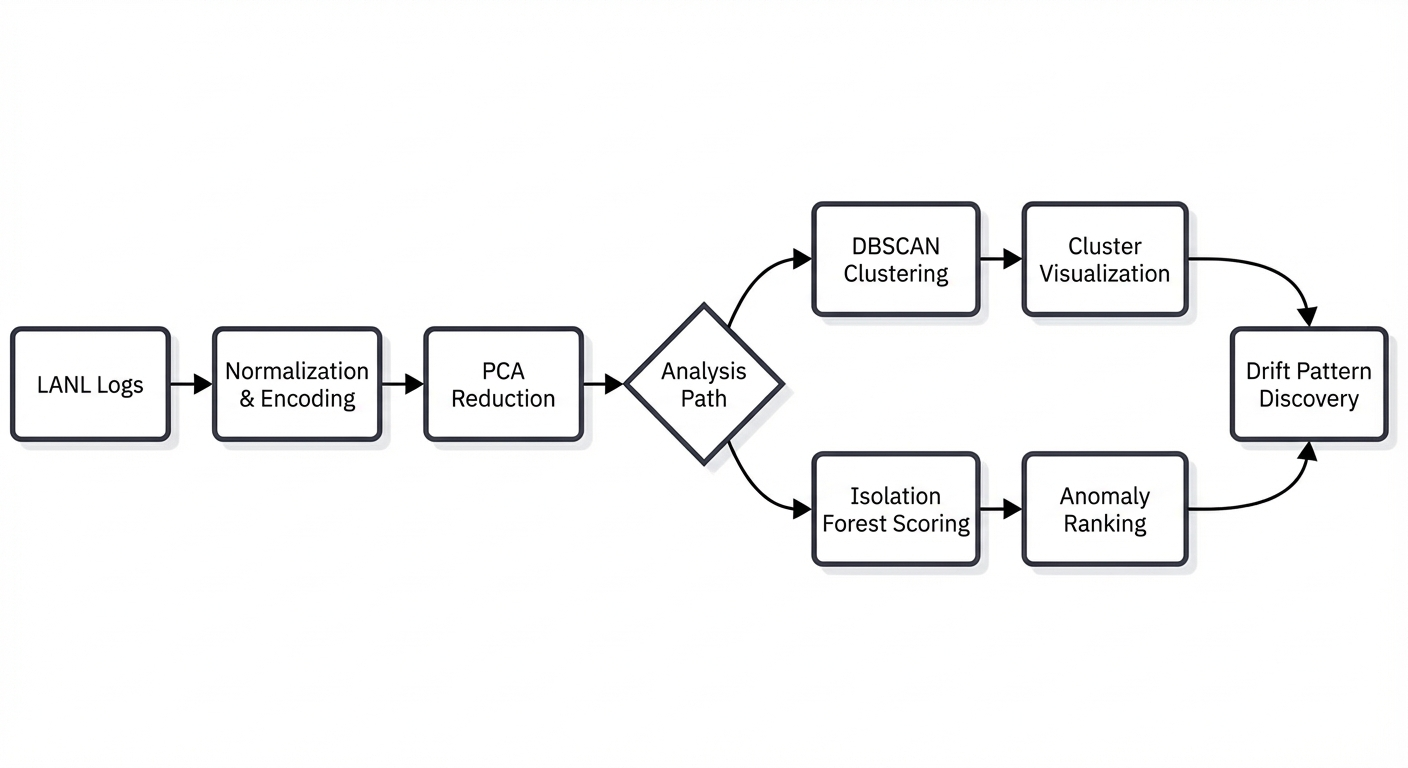
\includegraphics[height=6cm, width=0.9\textwidth]{pipeline.png}
    \caption{Data Mining Pipeline for Pattern Discovery.}
    \label{fig1}
\end{figure*}

\section{Planned Techniques}
Our analysis follows a three-stage pipeline for unsupervised learning.

\subsection{Dimensionality Reduction (PCA)}
PCA will be used to compress high-dimensional data into a smaller space. This helps us visualize behavior and see if drift shows up as movement away from the dense regions where normal activity occurs.

\subsection{Clustering (DBSCAN)}
We will use DBSCAN to find regions of normal behavior. We chose this because we do not need to tell it how many clusters to find. Points that do not relate to these regions are likely to represent drifting behavior.

\subsection{Anomaly Detection (Isolation Forest)}
Isolation Forests will be used to give anomaly scores to different events. If an event is easy to isolate with few splits, it gets a higher score. This gives us a way to rank potential drift cases for further investigation.

\section{Evaluation and Validation}
Evaluating unsupervised models is challenging due to the lack of direction/definition of an unwarranted connection. We will use the following metrics to validate our discoveries:

\subsection{Internal Evaluation}
We will utilize the Silhouette Coefficient and Davies-Bouldin Index to assess the cluster's quality, which we will then relate to the variables that we plan to extract from the datasets. A high Silhouette score will indicate the behavioral clusters as being well-defined and distinct, which suggests that the baseline is normal. Additionally, we will look for a low Davies-Bouldin Index because that will indicate a favorable ratio of within-cluster scatter to between-cluster separation. These metrics will be applied throughout our tuning phase as we utilize DBSCAN's epsilon and min\_samples parameters to establish a baseline understanding of the network activity. The purpose of using both metrics is to objectively determine the most applicable configuration that will return the most distinct behavioral groups before we delve into the anomaly detection itself. The Silhouette score is how we can understand the baseline behaviors, while the Davies-Bouldin score will allow us to visualize the distance/distinction of data clusters and Shadow IT points. 

\subsection{Anomaly Verification}
The anomalies that are identified by the Isolation Forest will be utilized for a qualitative observation. We will take these suspected anomalies and cross-reference high scoring outliers with the original LANL event logs. From this point we will be able to see if they correspond to known administrative patterns or harmless irregularities. 

\subsection{Conclusion}
The aim of this project is to ultimately create and demonstrate the ability to delimit behavioral analysis when regarding Attack Surface Drift. This will be identified through statistical deviations in the network telemetry by implementing a pipeline of PCA, DBSCAN, and Isolation Forests.  

\section{Preliminary Timeline}
\begin{itemize}
    \item Milestone 2: Download the data, sample it, and handle the feature encoding and normalization.
    \item Milestone 3: Apply PCA and DBSCAN, tune the parameters, and generate the anomaly scores.
    \item Milestone 4: Look at the high-scoring anomalies and see if the patterns actually represent meaningful drift.
\end{itemize}

\section{GitHub Repository}
Repository Name: \texttt{cs4412-asm-mining}
\url{https://github.com/asundby6/cs4412-asm-mining}

\begin{thebibliography}{0}
\bibitem{lanl-turcotte} 
M. Turcotte, A. Kent, and C. Hash, ``Unified Host and Network Data Set,'' in \textit{Data Science for Cyber-Security}, World Scientific, Nov. 2018, pp. 1--22. [Online]. Available: \url{https://csr.lanl.gov/data/2017/}
\end{thebibliography}

\end{document}